\chapter{Case}


\section{Situation Report}

The overall objective off all parties involved in this case was to configure and develop a system that could receive \gls{sms}-reports. 

\begin{figure}
\centering
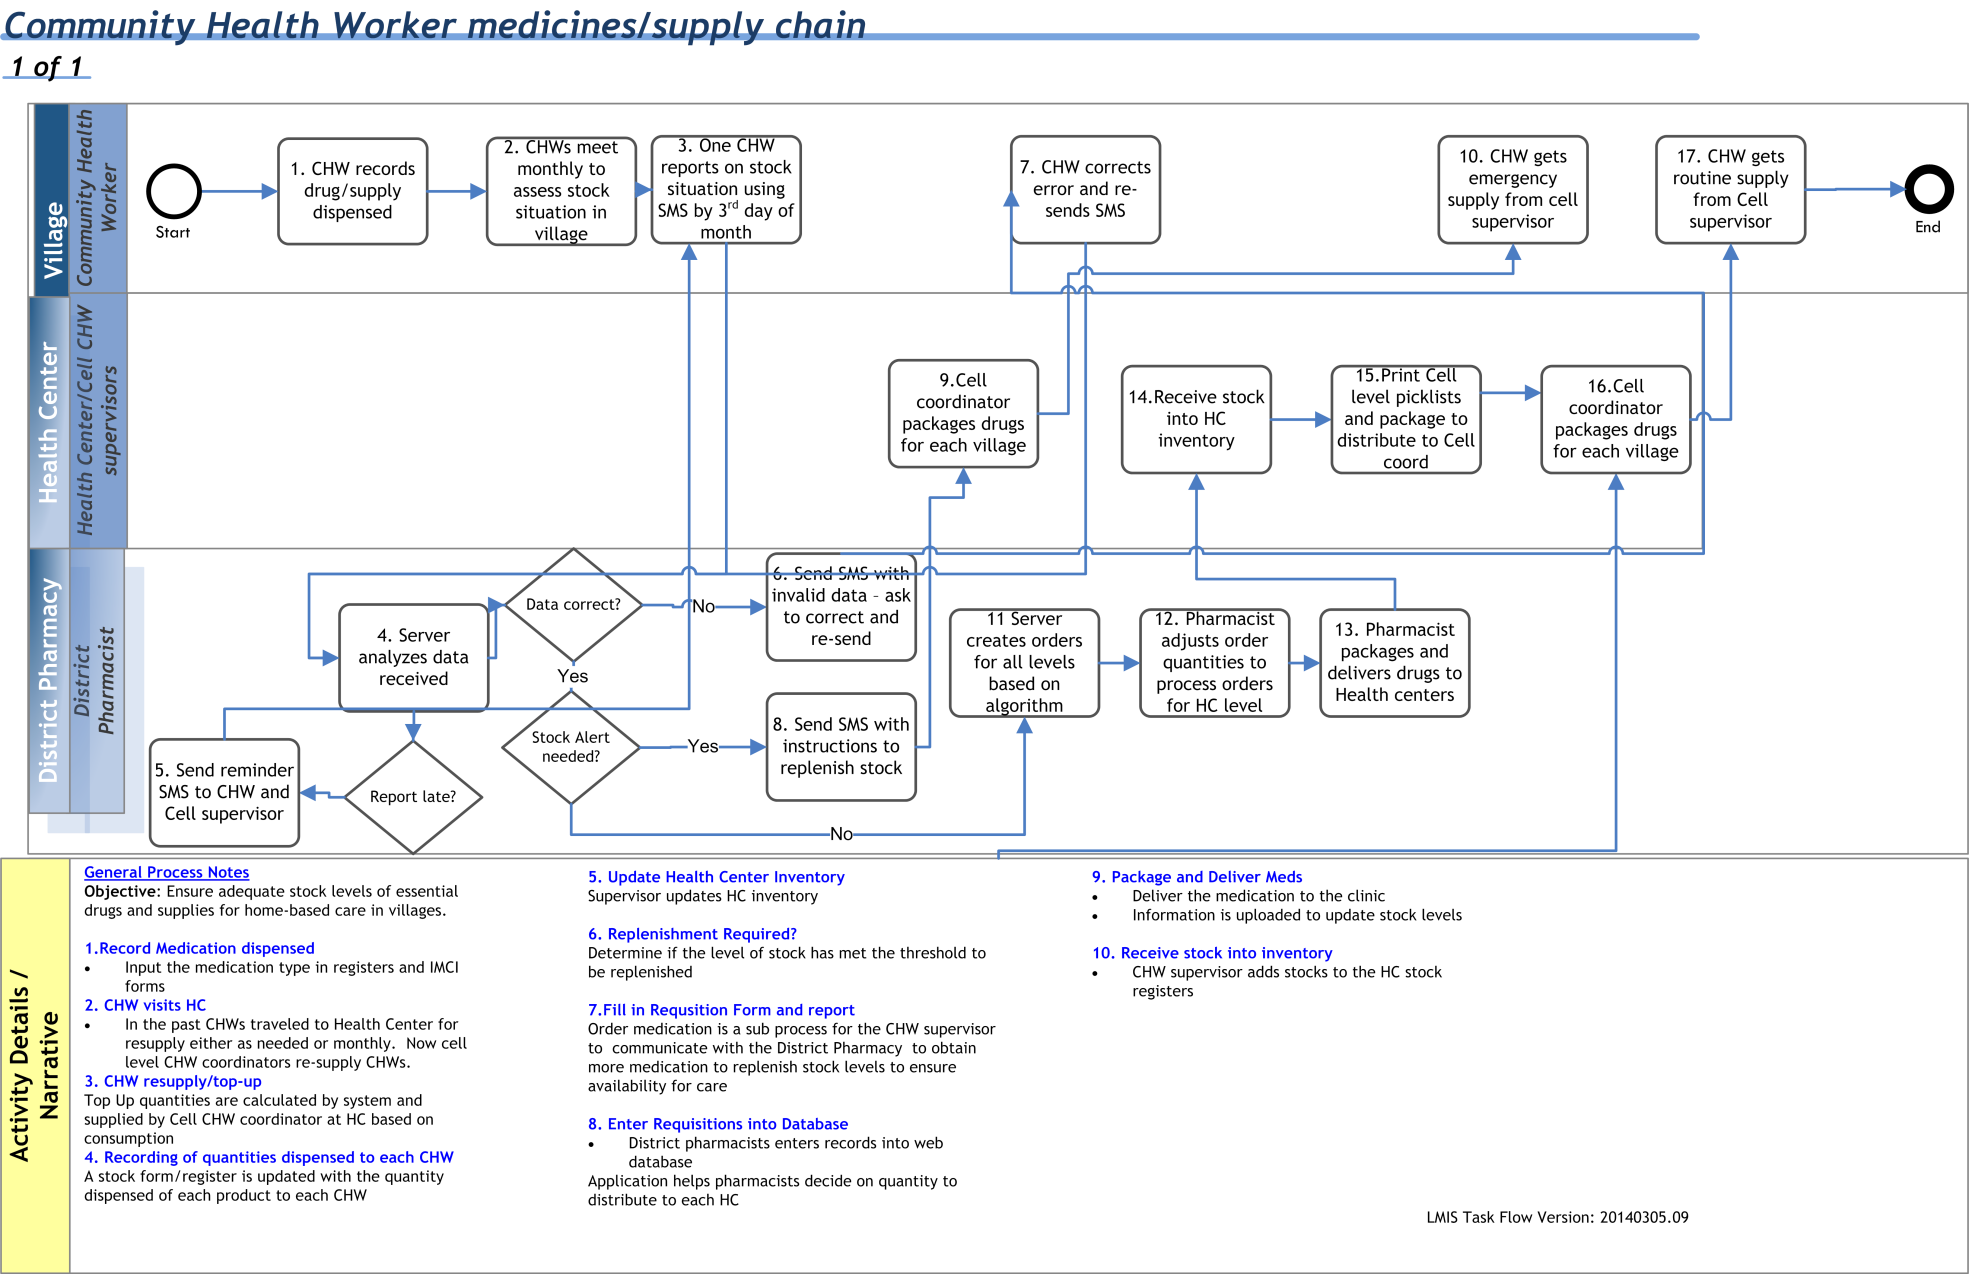
\includegraphics[width=\textwidth]{case/img/chwSupplyChainFuture}
\caption{\gls{chw} Supply Chain in the Future}
\label{chwSupplyChainPresent}
\end{figure}

\section{Diagnosis}

\subsection{Objectives}
We started out with four simple objectives. 

\begin{description}
\item[\#1] Send SMS and email notifications based on rules.
\item[\#2] Send SMS and email reminder if a report is more than 4 days delayed.
\item[\#3] If user data does not map correctly user feedback should be provided.
\item[\#4] A functional SMS based reporting system.
\end{description}

This was the basis for our case.

\subsection{Use Cases}

\begin{table}
	\centering
	\begin{tabular}{|p{5cm}|p{7cm}|}
		\hline
		\multicolumn{2}{|c|}{\textbf{Send SMS and Email Notifications}}\\
		\hline
		\textbf{Goal:} & Create orders\\
		\hline
		\textbf{Primary Actor:} & System\\
		\hline
		\multirow{3}{*}{\textbf{Secondary Actor:}}	& Cell CHW Supervisor \\
																								& HC CHW Supervisor \\ 
																								& District Pharmacist \\
		\hline
		\multirow{4}{*}{\textbf{Main Success Scenario:}}	& 1. CHW reports distributed and stock values. \\
																											& 2. System processes report. \\
																											& 3. System calculates essential drugs needed for each level. \\
																											& 4. System sends orders to cell, sector and district. \\
		\hline
		\textbf{Extensions:} & \\
		\hline
	\end{tabular}
	\caption{Textual Use Case: Send SMS and Email Notifications}
	\label{tab:notifications}
\end{table}


\begin{table}
	\centering
	\begin{tabular}{|p{5cm}|p{7cm}|}
		\hline
		\multicolumn{2}{|c|}{\textbf{Send SMS and Email Reminders}}\\
		\hline
		\textbf{Goal:} & Send reminder \\
		\hline
		\textbf{Primary Actor:} & System \\
		\hline
		\multirow{2}{*}{\textbf{Secondary Actor:}}	& CHW \\
																								& Cell CHW Supervisor \\
		\hline
		\multirow{5}{*}{\textbf{Main Success Scenario:}}	& 1. CHW misses report deadline. \\
																											& 2. 5 days goes by. \\
																											& 3. System sends reminder by email and SMS. \\
																											& 4. Another 5 days goes by. \\
																											& 5. System sends reminder by email and SMS. \\
																											
		\hline
		\textbf{Extensions:} & \\
		\hline
	\end{tabular}
	\caption{Textual Use Case: Send SMS and Email Reminders}
	\label{tab:reminders}
\end{table}


\begin{table}
	\centering
	\begin{tabular}{|p{5cm}|p{7cm}|}
		\hline
		\multicolumn{2}{|c|}{\textbf{Send Report Feedback}} \\
		\hline
		\textbf{Goal:} & Process SMS message\\
		\hline
		\textbf{Primary Actor:} & System \\
		\hline
		\textbf{Secondary Actor:} & Community Health Worker \\
		\hline
		\multirow{6}{*}{\textbf{Main Success Scenario:}}	& 1. CHW reports data incorrectly by SMS. \\
																											& 2. System receives SMS. \\
																											& 3. SMS triggers feedback message. \\
																											& 4. CHW corrects message and re-sends report. \\
																											& 5. System processes SMS. \\
																											& 6. System updates database. \\
		\hline
		\textbf{Extensions:} & \\
		\hline
	\end{tabular}
	\caption{Textual Use Case: Send Report Feedback}
	\label{tab:feedback}
\end{table}

\begin{table}
	\centering
	\begin{tabular}{|p{5cm}|p{7cm}|}
		\hline
		\multicolumn{2}{|c|}{\textbf{Report Using SMS}}\\
		\hline
		\textbf{Goal:} & Update Database \\
		\hline
		\textbf{Primary Actor:} & Community Health Worker\\
		\hline
		\textbf{Secondary Actor:} & System \\
		\hline
		\multirow{5}{*}{\textbf{Main Success Scenario:}}	& 1. CHW reports stock and distributed values of essential drugs. \\
																											& 2. System receives SMS. \\
																											& 3. System processes SMS. \\
																											& 4. System updates database. \\
																											& 5. System sends confirmation SMS to CHW. \\
		\hline
		\textbf{Extensions:} & \\
		\hline
	\end{tabular}
	\caption{Textual Use Case: Report Using SMS}
	\label{tab:smsreport}
\end{table}

Based on the four objectives we made four use cases that was supposed to represent each one. Objective \#1 would be represented with use case \ref{tab:notifications}, objective \#2 with \ref{tab:reminders}, \#3 with \ref{tab:feedback} and \#4 with \ref{tab:smsreport}. These use cases worked as guidelines for our further work. They were not updated later on, because of the continuous updated requirements from \gls{chd} and other co-workers. That is one of the key characterizations of this project. The requirements kept on updating as more and more people got involved in the process. The more progress we made the less progress we made. As the project was coming more and more realized, more interest were made to the project, and more requirements were added. There were a kind of common understanding in the team. Once you got the picture, you didn't need to operate on a model anymore. Everyone kinda knew what needed to be done. The result of the diagnosis were essentially a clarification of what we were supposed to do and who are involved. The clients are \gls{chd}. A meeting took place and a list of contact information was exchanged. The users of the system are \gls{chw}'s, Cell \gls{chw} Supervisors, \gls{hc} \gls{chw} Supervisors and District Pharmacists. The basic idea is that the \gls{chd} would like to have \gls{hmis} make a system that enables \gls{chw}'s to report using \gls{sms} and based on this have automatic generated orders sent to the \gls{hc}'s and District Pharmacists.

\subsection{Planning}


\subsection{Re-Supply Algorithm}

\begin{equation}
stk_{n} = stk_{n-1} + rcd_{n} - disp_{n}
\end{equation}

\begin{eqnarray}
reorder_{n} & = & (amc_{n} \cdot 2) - stk_{n} \\
amc_{n} & = & \frac{disp_{n-2} + disp_{n-1} + disp_{n}}{3} \\
disp_{n} & = & stk_{n-1} + rcd_{n} - stk_{n} \\
disp_{n-1} & = & stk_{n-2} + rcd_{n-1} - stk_{n-1} \\
disp_{n-2} & = & stk_{n-3} + rcd_{n-2} - stk_{n-2}
\end{eqnarray}


\begin{description}
\item[$reorder_{n}$]
This variable represents the quantity of how much is needed at the next re-supply of one village. $n$ in this case represents the last month. If in May, it represents reorder quantity for the end of month of April.
\item[$amc_{n}$]
Represents the average monthly consumption based on the last 3 months in one village. I in May, that would be the average monthly consumption based on February, March and April.
\item[$disp_{n}$]
This variable is calculated based on the the values reported and is the number of items distributed by one village during one month.
\item[$stk_{n}$]
The quantity in stock at the end of the month of one village. Usually reported within 1--5 days into the next month it represents. Stock in April is usually reported between 1st and 5th of May.
\item[$rcd_{n}$]
This variable is the sum of items received in one village during the month it represents. If a \gls{chw} receives 10 condoms 2nd of April, it should be reported the same day. If a village receives another 10 condoms the 13th of April, that should also be reported the same day it is received. $rcd_{n}$ for April would then be the sum of those values, 20.
\begin{equation}
rcd_{n} = \sum_{k = 1}^{j} rcd_{n,k}
\label{eq:received}
\end{equation}.
A more mathematical description in equation \ref{eq:received}, where j represents the number of days in the month.
\end{description}